\documentclass{article}
\usepackage[margin=0.8cm]{geometry}
\usepackage{amsmath,amssymb}
\usepackage{xcolor}
\usepackage{tikz}
\usepackage{pgfplots}
\usepgfplotslibrary{groupplots,fillbetween,colormaps}
\usetikzlibrary{arrows.meta,positioning,calc}
\pgfplotsset{compat=1.18}
\definecolor{papBlue}{HTML}{1f77b4}
\definecolor{papOrange}{HTML}{ff7f0e}
\definecolor{papGreen}{HTML}{2ca02c}
\definecolor{papRed}{HTML}{d62728}
\definecolor{papPurple}{HTML}{9467bd}
\definecolor{papTeal}{HTML}{17becf}
\definecolor{papGold}{HTML}{bcbd22}
\definecolor{papGray}{HTML}{7f7f7f}
\pgfplotsset{paperaxis/.style={width=0.95\linewidth,height=0.62\linewidth,grid=major,grid style={draw=papGray!20}}}

\begin{document}
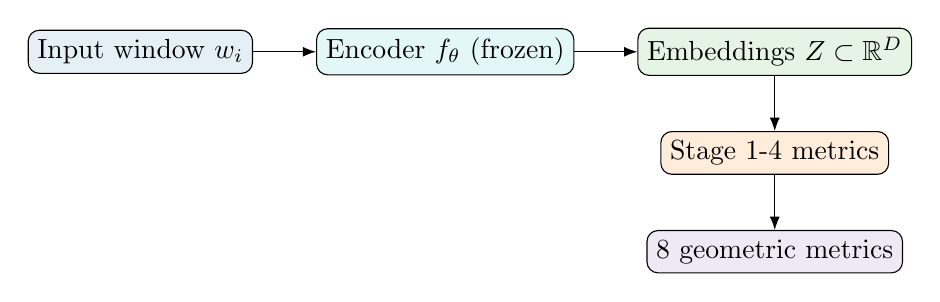
\begin{tikzpicture}[>=Latex,node distance=7mm and 8mm]
\node[draw,rounded corners,fill=papBlue!12] (a) {Input window $w_i$};
\node[draw,rounded corners,fill=papTeal!12,right=of a] (b) {Encoder $f_\theta$ (frozen)};
\node[draw,rounded corners,fill=papGreen!12,right=of b] (c) {Embeddings $Z\subset\mathbb{R}^D$};
\node[draw,rounded corners,fill=papOrange!15,below=of c] (d) {Stage 1-4 metrics};
\node[draw,rounded corners,fill=papPurple!15,below=of d] (e) {8 geometric metrics};
\draw[->] (a)--(b);\draw[->] (b)--(c);\draw[->] (c)--(d);\draw[->] (d)--(e);
\end{tikzpicture}
\newpage
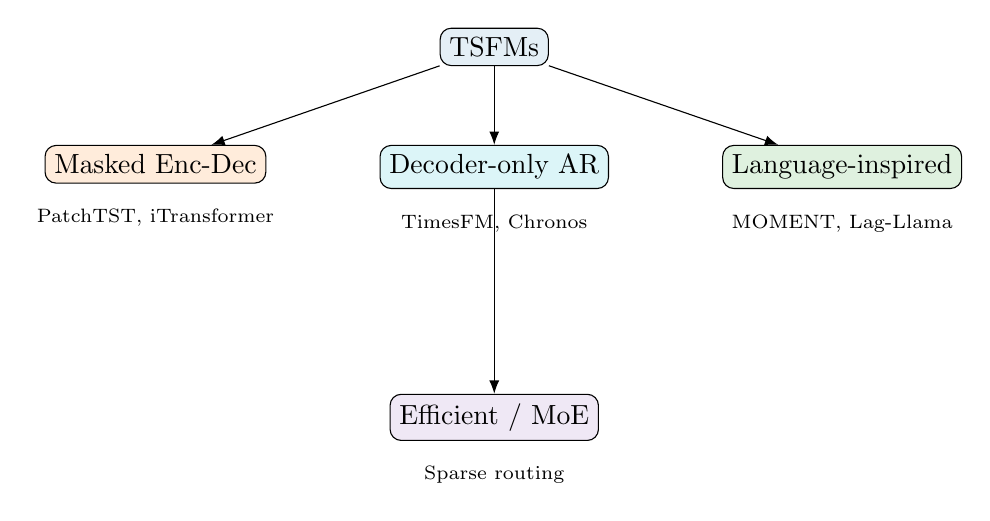
\begin{tikzpicture}[>=Latex,node distance=7mm and 8mm]
\node[draw,rounded corners,fill=papBlue!12] (r) {TSFMs};
\node[draw,rounded corners,fill=papOrange!15,below left=10mm and 22mm of r] (a) {Masked Enc-Dec};
\node[draw,rounded corners,fill=papTeal!15,below=10mm of r] (b) {Decoder-only AR};
\node[draw,rounded corners,fill=papGreen!15,below right=10mm and 22mm of r] (c) {Language-inspired};
\node[draw,rounded corners,fill=papPurple!15,below=26mm of b] (d) {Efficient / MoE};
\node[font=\scriptsize,below=2mm of a] {PatchTST, iTransformer};
\node[font=\scriptsize,below=2mm of b] {TimesFM, Chronos};
\node[font=\scriptsize,below=2mm of c] {MOMENT, Lag-Llama};
\node[font=\scriptsize,below=2mm of d] {Sparse routing};
\draw[->] (r)--(a);\draw[->] (r)--(b);\draw[->] (r)--(c);\draw[->] (b)--(d);
\end{tikzpicture}
\newpage
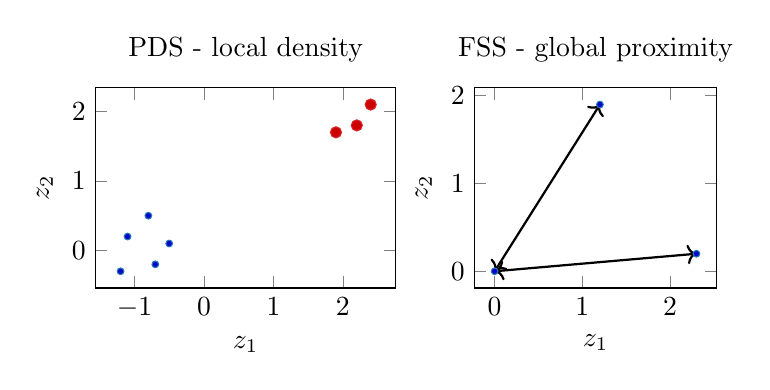
\begin{tikzpicture}
\begin{groupplot}[group style={group size=2 by 1,horizontal sep=1.0cm},width=0.45\linewidth,height=0.34\linewidth]
\nextgroupplot[title={PDS - local density},axis equal image,xlabel={$z_1$},ylabel={$z_2$}]
\addplot+[only marks,mark=*,mark size=1.2pt,color=papBlue] coordinates {(-1.1,0.2) (-0.8,0.5) (-0.5,0.1) (-0.7,-0.2) (-1.2,-0.3)};
\addplot+[only marks,mark=*,mark size=2pt,color=papRed] coordinates {(2.2,1.8) (2.4,2.1) (1.9,1.7)};
\nextgroupplot[title={FSS - global proximity},axis equal image,xlabel={$z_1$},ylabel={$z_2$}]
\addplot+[only marks,mark=*,mark size=1.2pt,color=papBlue] coordinates {(0,0) (2.3,0.2) (1.2,1.9)};
\draw[<->,thick] (axis cs:0,0)--(axis cs:2.3,0.2);
\draw[<->,thick] (axis cs:0,0)--(axis cs:1.2,1.9);
\end{groupplot}
\end{tikzpicture}
\newpage
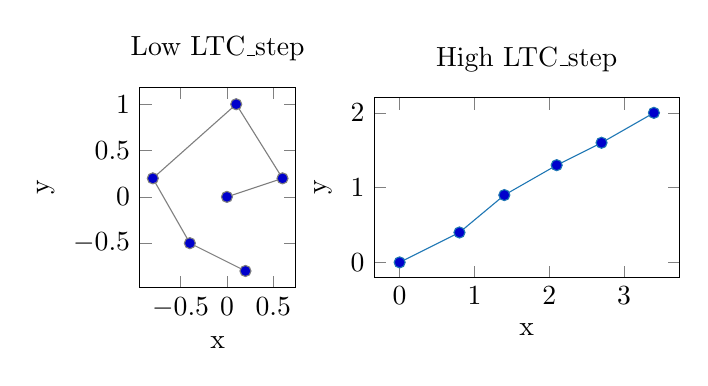
\begin{tikzpicture}
\begin{groupplot}[group style={group size=2 by 1,horizontal sep=1.0cm},width=0.45\linewidth,height=0.34\linewidth,axis equal image]
\nextgroupplot[title={Low LTC\_step},xlabel=x,ylabel=y]
\addplot+[mark=*,color=papGray] coordinates {(0,0) (0.6,0.2) (0.1,1.0) (-0.8,0.2) (-0.4,-0.5) (0.2,-0.8)};
\nextgroupplot[title={High LTC\_step},xlabel=x,ylabel=y]
\addplot+[mark=*,color=papBlue] coordinates {(0,0) (0.8,0.4) (1.4,0.9) (2.1,1.3) (2.7,1.6) (3.4,2.0)};
\end{groupplot}
\end{tikzpicture}
\newpage
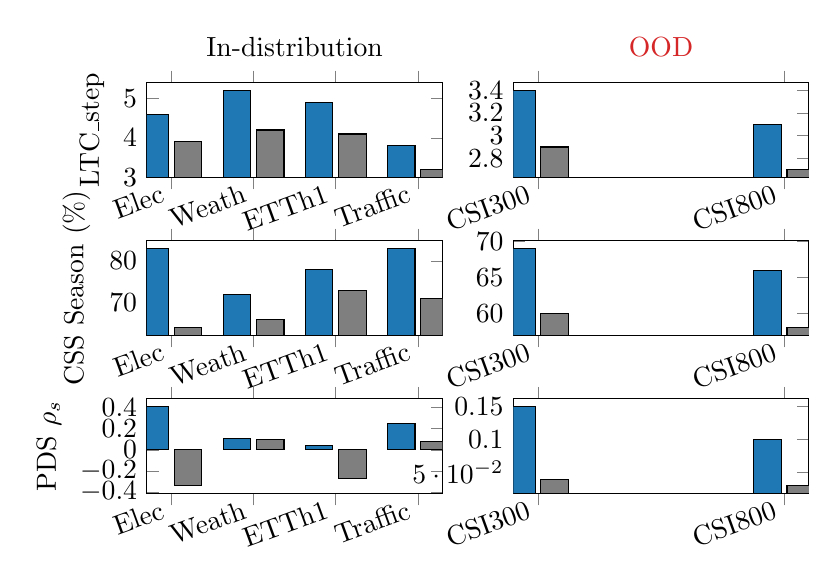
\begin{tikzpicture}
\begin{groupplot}[group style={group size=2 by 3,horizontal sep=0.9cm,vertical sep=0.8cm},width=0.44\linewidth,height=0.23\linewidth,ybar,symbolic x coords={Elec,Weath,ETTh1,Traffic},xtick=data,xticklabel style={rotate=20,anchor=east}]
\nextgroupplot[title={In-distribution},ylabel={LTC\_step}]\addplot[fill=papBlue] coordinates {(Elec,4.6) (Weath,5.2) (ETTh1,4.9) (Traffic,3.8)};\addplot[fill=papGray] coordinates {(Elec,3.9) (Weath,4.2) (ETTh1,4.1) (Traffic,3.2)};
\nextgroupplot[title={OOD},symbolic x coords={CSI300,CSI800},xtick=data,title style={text=papRed}]\addplot[fill=papBlue] coordinates {(CSI300,3.4) (CSI800,3.1)};\addplot[fill=papGray] coordinates {(CSI300,2.9) (CSI800,2.7)};
\nextgroupplot[ylabel={CSS Season (\%)}]\addplot[fill=papBlue] coordinates {(Elec,83) (Weath,72) (ETTh1,78) (Traffic,83)};\addplot[fill=papGray] coordinates {(Elec,64) (Weath,66) (ETTh1,73) (Traffic,71)};
\nextgroupplot[symbolic x coords={CSI300,CSI800},xtick=data]\addplot[fill=papBlue] coordinates {(CSI300,69) (CSI800,66)};\addplot[fill=papGray] coordinates {(CSI300,60) (CSI800,58)};
\nextgroupplot[ylabel={PDS $\rho_s$}]\addplot[fill=papBlue] coordinates {(Elec,0.41) (Weath,0.11) (ETTh1,0.04) (Traffic,0.25)};\addplot[fill=papGray] coordinates {(Elec,-0.34) (Weath,0.10) (ETTh1,-0.27) (Traffic,0.08)};
\nextgroupplot[symbolic x coords={CSI300,CSI800},xtick=data]\addplot[fill=papBlue] coordinates {(CSI300,0.15) (CSI800,0.10)};\addplot[fill=papGray] coordinates {(CSI300,0.04) (CSI800,0.03)};
\end{groupplot}
\end{tikzpicture}
\newpage
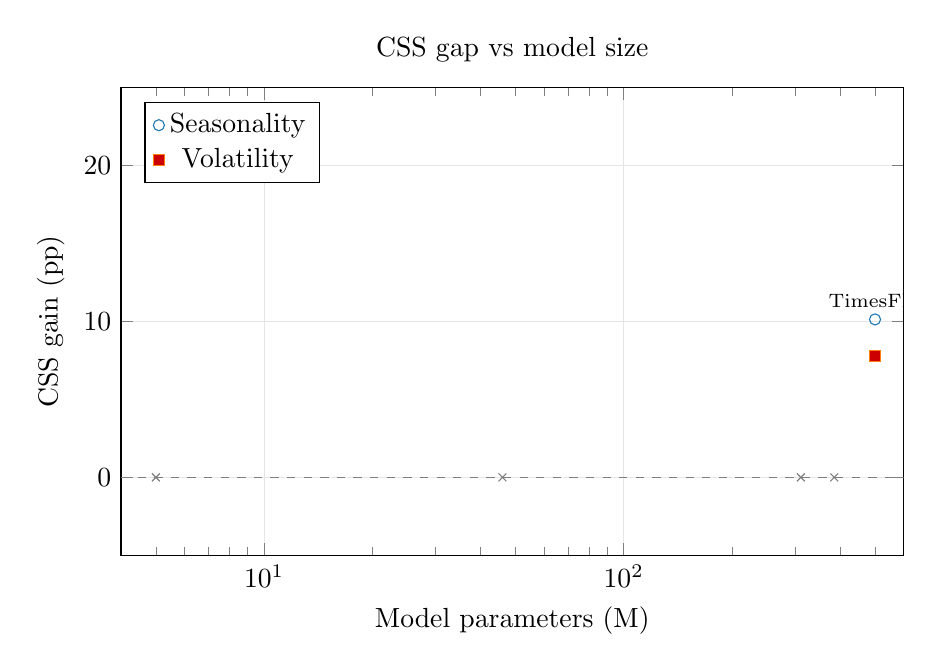
\begin{tikzpicture}
\begin{axis}[paperaxis,xmode=log,xmin=4,xmax=600,ymin=-5,ymax=25,xlabel={Model parameters (M)},ylabel={CSS gain (pp)},legend pos=north west,title={CSS gap vs model size}]
\addplot+[only marks,mark=o,color=papBlue] coordinates {(500,10.139)};\addlegendentry{Seasonality}
\addplot+[only marks,mark=square*,color=papOrange] coordinates {(500,7.815)};\addlegendentry{Volatility}
\addplot+[only marks,mark=x,color=papGray] coordinates {(5,0) (46,0) (385,0) (311,0)};
\node[font=\scriptsize] at (axis cs:500,11.339) {TimesFM};
\addplot[dashed,color=papGray] coordinates {(4,0) (600,0)};
\end{axis}
\end{tikzpicture}
\newpage
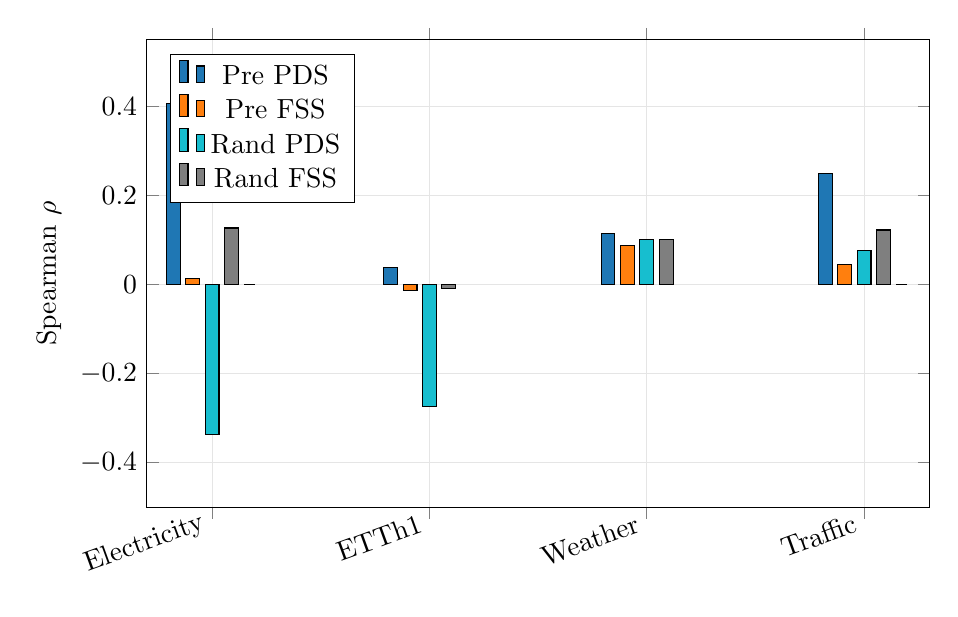
\begin{tikzpicture}
\begin{axis}[paperaxis,ybar,bar width=5pt,xtick={0,1,2,3},xticklabels={Electricity,ETTh1,Weather,Traffic},x tick label style={rotate=20,anchor=east},ylabel={Spearman $\rho$},legend pos=north west,ymin=-0.5,ymax=0.55]
\addplot[fill=papBlue] coordinates {(0,0.4064) (1,0.0387) (2,0.1142) (3,0.2502)};\addlegendentry{Pre PDS}
\addplot[fill=papOrange] coordinates {(0,0.0128) (1,-0.0125) (2,0.0876) (3,0.0452)};\addlegendentry{Pre FSS}
\addplot[fill=papTeal] coordinates {(0,-0.3376) (1,-0.2732) (2,0.1018) (3,0.0769)};\addlegendentry{Rand PDS}
\addplot[fill=papGray] coordinates {(0,0.1271) (1,-0.0092) (2,0.1008) (3,0.1227)};\addlegendentry{Rand FSS}
\addplot[dashed] coordinates {(0,0) (3,0)};
\end{axis}
\end{tikzpicture}
\newpage
\input{fig_geodesic_reliability_seed_sweep_check.tex}\newpage
\input{fig_geodesic_reliability_seed_sweep_best.tex}\newpage
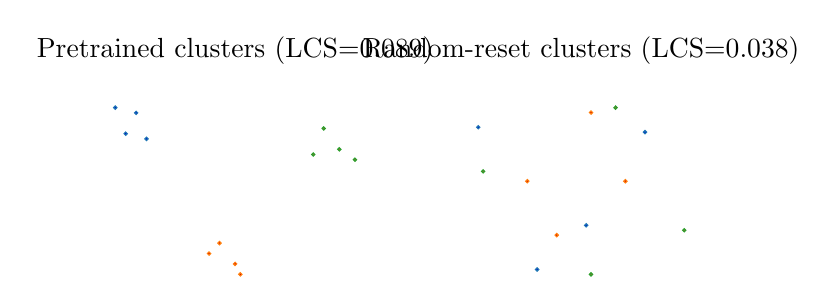
\begin{tikzpicture}
\begin{groupplot}[group style={group size=2 by 1,horizontal sep=1.0cm},width=0.45\linewidth,height=0.34\linewidth,axis equal image,axis lines=none]
\nextgroupplot[title={Pretrained clusters (LCS=0.089)}]
\addplot+[only marks,mark=*,mark size=0.6pt,color=papBlue] coordinates {(-2,1.3) (-1.8,1.7) (-2.2,1.8) (-1.6,1.2)};
\addplot+[only marks,mark=*,mark size=0.6pt,color=papOrange] coordinates {(0.1,-1.2) (-0.4,-1.0) (0.2,-1.4) (-0.2,-0.8)};
\addplot+[only marks,mark=*,mark size=0.6pt,color=papGreen] coordinates {(2.1,1.0) (1.8,1.4) (2.4,0.8) (1.6,0.9)};
\nextgroupplot[title={Random-reset clusters (LCS=0.038)}]
\addplot+[only marks,mark=*,mark size=0.6pt,color=papBlue] coordinates {(-2,1.3) (0.2,-0.7) (1.4,1.2) (-0.8,-1.6)};
\addplot+[only marks,mark=*,mark size=0.6pt,color=papOrange] coordinates {(1.0,0.2) (-1.0,0.2) (0.3,1.6) (-0.4,-0.9)};
\addplot+[only marks,mark=*,mark size=0.6pt,color=papGreen] coordinates {(2.2,-0.8) (-1.9,0.4) (0.8,1.7) (0.3,-1.7)};
\end{groupplot}
\end{tikzpicture}
\newpage
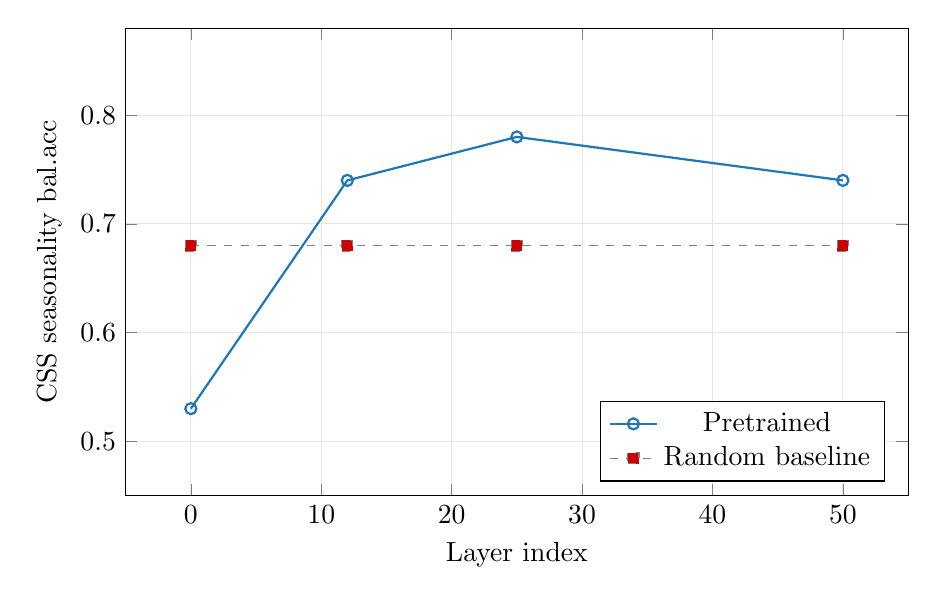
\begin{tikzpicture}
\begin{axis}[paperaxis,xlabel={Layer index},ylabel={CSS seasonality bal.acc},legend pos=south east,ymin=0.45,ymax=0.88]
\addplot+[mark=o,color=papBlue,thick] coordinates {(0,0.53) (12,0.74) (25,0.78) (50,0.74)};\addlegendentry{Pretrained}
\addplot+[mark=square*,color=papGray,dashed] coordinates {(0,0.68) (12,0.68) (25,0.68) (50,0.68)};\addlegendentry{Random baseline}
\end{axis}
\end{tikzpicture}
\newpage
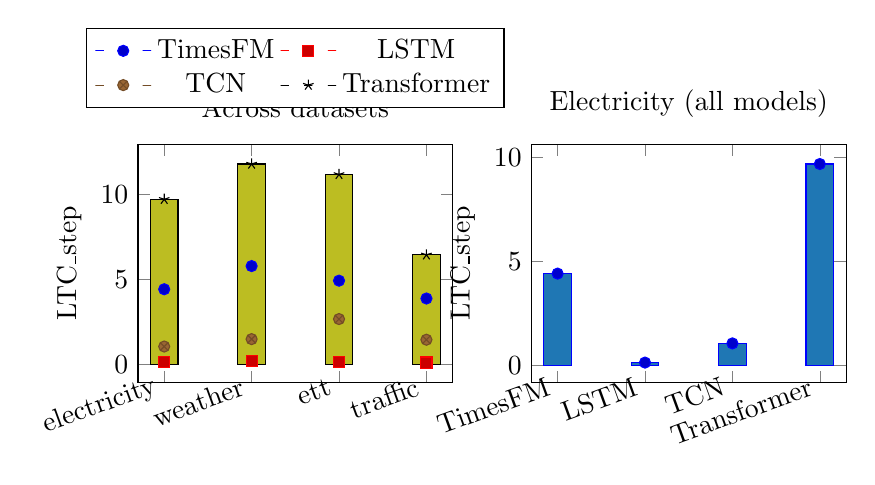
\begin{tikzpicture}
\begin{groupplot}[group style={group size=2 by 1,horizontal sep=1.0cm},width=0.46\linewidth,height=0.38\linewidth,ylabel={LTC\_step},symbolic x coords={electricity,weather,ett,traffic},xtick=data,xticklabel style={rotate=20,anchor=east}]
\nextgroupplot[title={Across datasets},legend style={at={(0.5,1.15)},anchor=south,legend columns=2}]
\addplot+[ybar,fill=papBlue] coordinates {(electricity,4.415) (weather,5.775) (ett,4.918) (traffic,3.871)};\addlegendentry{TimesFM}
\addplot+[ybar,fill=papGray] coordinates {(electricity,0.127) (weather,0.186) (ett,0.139) (traffic,0.109)};\addlegendentry{LSTM}
\addplot+[ybar,fill=papTeal] coordinates {(electricity,1.052) (weather,1.486) (ett,2.664) (traffic,1.451)};\addlegendentry{TCN}
\addplot+[ybar,fill=papGold] coordinates {(electricity,9.697) (weather,11.767) (ett,11.156) (traffic,6.435)};\addlegendentry{Transformer}
\nextgroupplot[title={Electricity (all models)},symbolic x coords={TimesFM,LSTM,TCN,Transformer},xtick=data]
\addplot+[ybar,fill=papBlue] coordinates {(TimesFM,4.415) (LSTM,0.127) (TCN,1.052) (Transformer,9.697)};
\end{groupplot}
\end{tikzpicture}
\newpage
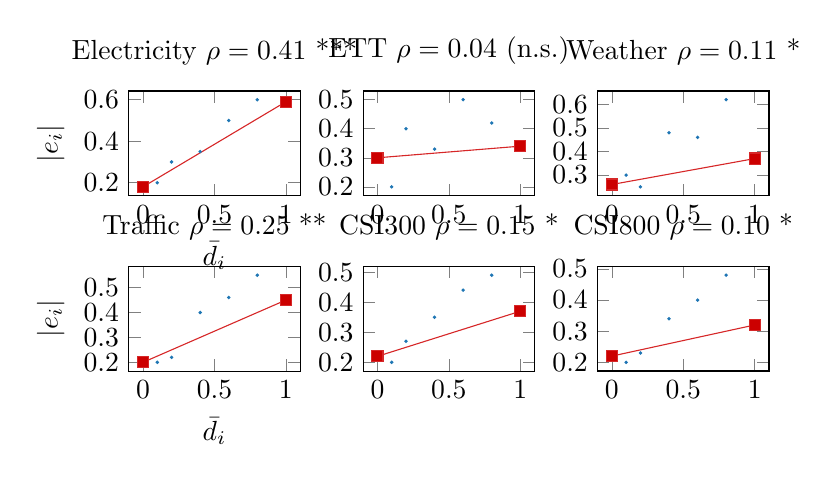
\begin{tikzpicture}
\begin{groupplot}[group style={group size=3 by 2,horizontal sep=0.8cm,vertical sep=0.9cm},width=0.31\linewidth,height=0.24\linewidth]
\nextgroupplot[title={Electricity\ $\rho=0.41$ ***},xlabel={$\bar d_i$},ylabel={$|e_i|$}]\addplot+[only marks,mark=*,mark size=0.4pt,color=papBlue] coordinates {(0.1,0.2) (0.2,0.3) (0.4,0.35) (0.6,0.5) (0.8,0.6)};\addplot+[domain=0:1,samples=2,color=papRed] {0.41*x+0.18};
\nextgroupplot[title={ETT\ $\rho=0.04$ (n.s.)}]\addplot+[only marks,mark=*,mark size=0.4pt,color=papBlue] coordinates {(0.1,0.2) (0.2,0.4) (0.4,0.33) (0.6,0.5) (0.8,0.42)};\addplot+[domain=0:1,samples=2,color=papRed] {0.04*x+0.30};
\nextgroupplot[title={Weather\ $\rho=0.11$ *}]\addplot+[only marks,mark=*,mark size=0.4pt,color=papBlue] coordinates {(0.1,0.3) (0.2,0.25) (0.4,0.48) (0.6,0.46) (0.8,0.62)};\addplot+[domain=0:1,samples=2,color=papRed] {0.11*x+0.26};
\nextgroupplot[title={Traffic\ $\rho=0.25$ **},xlabel={$\bar d_i$},ylabel={$|e_i|$}]\addplot+[only marks,mark=*,mark size=0.4pt,color=papBlue] coordinates {(0.1,0.2) (0.2,0.22) (0.4,0.4) (0.6,0.46) (0.8,0.55)};\addplot+[domain=0:1,samples=2,color=papRed] {0.25*x+0.20};
\nextgroupplot[title={CSI300\ $\rho=0.15$ *}]\addplot+[only marks,mark=*,mark size=0.4pt,color=papBlue] coordinates {(0.1,0.2) (0.2,0.27) (0.4,0.35) (0.6,0.44) (0.8,0.49)};\addplot+[domain=0:1,samples=2,color=papRed] {0.15*x+0.22};
\nextgroupplot[title={CSI800\ $\rho=0.10$ *}]\addplot+[only marks,mark=*,mark size=0.4pt,color=papBlue] coordinates {(0.1,0.2) (0.2,0.23) (0.4,0.34) (0.6,0.40) (0.8,0.48)};\addplot+[domain=0:1,samples=2,color=papRed] {0.10*x+0.22};
\end{groupplot}
\end{tikzpicture}
\newpage
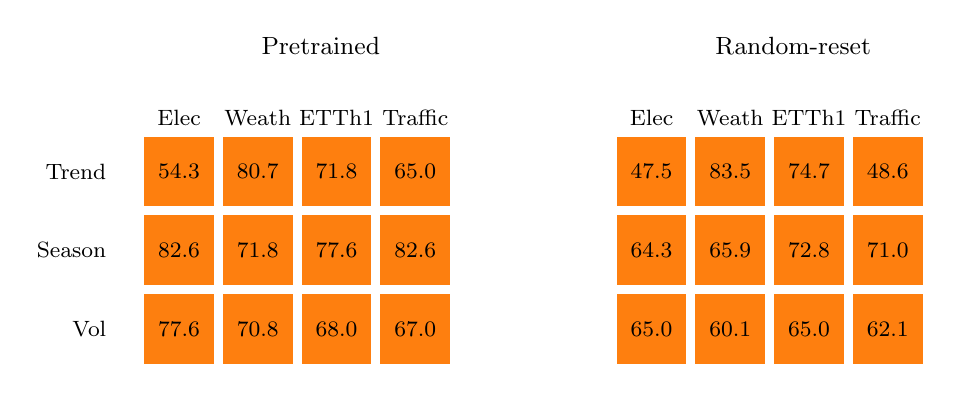
\begin{tikzpicture}[font=\footnotesize]
  % left block: pretrained
  \node[font=\small] at (1.8,3.6) {Pretrained};
  \foreach \x/\lab in {0/Elec,1/Weath,2/ETTh1,3/Traffic}{
    \node[anchor=north] at (\x,2.9) {\lab};
  }
  \foreach \y/\lab in {2/Trend,1/Season,0/Vol}{
    \node[anchor=east] at (-0.8,\y) {\lab};
  }
  \foreach \x/\y/\v in {
    0/2/54.3,1/2/80.7,2/2/71.8,3/2/65.0,
    0/1/82.6,1/1/71.8,2/1/77.6,3/1/82.6,
    0/0/77.6,1/0/70.8,2/0/68.0,3/0/67.0}{
    \pgfmathsetmacro{\shade}{(\v-40)/50}
    \fill[papBlue!\shade!papOrange,draw=white] (\x-0.45,\y-0.45) rectangle (\x+0.45,\y+0.45);
    \node at (\x,\y) {\v};
  }

  % right block: random-reset
  \begin{scope}[xshift=6.0cm]
    \node[font=\small] at (1.8,3.6) {Random-reset};
    \foreach \x/\lab in {0/Elec,1/Weath,2/ETTh1,3/Traffic}{
      \node[anchor=north] at (\x,2.9) {\lab};
    }
    \foreach \x/\y/\v in {
      0/2/47.5,1/2/83.5,2/2/74.7,3/2/48.6,
      0/1/64.3,1/1/65.9,2/1/72.8,3/1/71.0,
      0/0/65.0,1/0/60.1,2/0/65.0,3/0/62.1}{
      \pgfmathsetmacro{\shade}{(\v-40)/50}
      \fill[papBlue!\shade!papOrange,draw=white] (\x-0.45,\y-0.45) rectangle (\x+0.45,\y+0.45);
      \node at (\x,\y) {\v};
    }
  \end{scope}
\end{tikzpicture}
\newpage
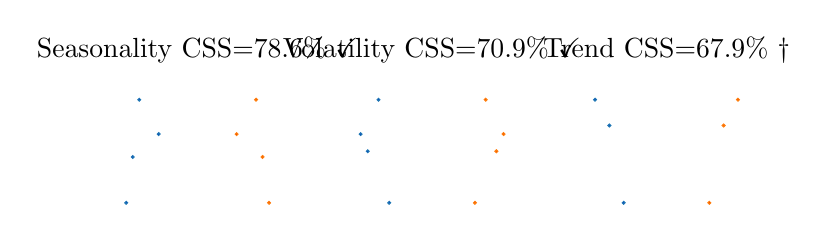
\begin{tikzpicture}
\begin{groupplot}[group style={group size=3 by 1,horizontal sep=0.8cm},width=0.31\linewidth,height=0.26\linewidth,axis lines=none]
\nextgroupplot[title={Seasonality\ CSS=78.6\% \checkmark}]
\addplot+[only marks,mark=*,mark size=0.5pt,color=papBlue] coordinates {(-2,0) (-1.8,0.5) (-2.2,-0.4) (-1.2,0.2)};
\addplot+[only marks,mark=*,mark size=0.5pt,color=papOrange] coordinates {(2,0) (1.8,0.5) (2.2,-0.4) (1.2,0.2)};
\nextgroupplot[title={Volatility\ CSS=70.9\% \checkmark}]
\addplot+[only marks,mark=*,mark size=0.5pt,color=papBlue] coordinates {(-1.8,0.2) (-1.2,-0.4) (-2.0,0.4) (-1.5,0.8)};
\addplot+[only marks,mark=*,mark size=0.5pt,color=papOrange] coordinates {(1.8,0.2) (1.2,-0.4) (2.0,0.4) (1.5,0.8)};
\nextgroupplot[title={Trend\ CSS=67.9\% $\dagger$}]
\addplot+[only marks,mark=*,mark size=0.5pt,color=papBlue] coordinates {(-0.8,0.2) (-0.6,-0.4) (-1.0,0.4)};
\addplot+[only marks,mark=*,mark size=0.5pt,color=papOrange] coordinates {(0.8,0.2) (0.6,-0.4) (1.0,0.4)};
\end{groupplot}
\end{tikzpicture}
\newpage
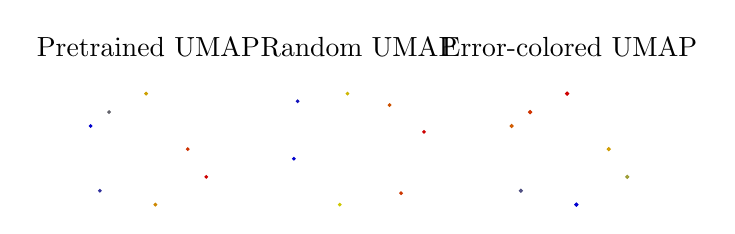
\begin{tikzpicture}
\begin{groupplot}[group style={group size=3 by 1,horizontal sep=0.8cm},width=0.31\linewidth,height=0.27\linewidth,axis equal image,axis lines=none]
\nextgroupplot[title={Pretrained UMAP}]\addplot+[only marks,mark=*,mark size=0.45pt,scatter,scatter src=x] coordinates {(-1,0.7) (-0.6,1.0) (0.2,1.4) (1.1,0.2) (1.5,-0.4) (0.4,-1.0) (-0.8,-0.7)};
\nextgroupplot[title={Random UMAP}]\addplot+[only marks,mark=*,mark size=0.45pt,scatter,scatter src=x] coordinates {(-1.6,1.2) (-0.3,1.4) (0.8,1.1) (1.7,0.4) (1.1,-1.2) (-0.5,-1.5) (-1.7,-0.3)};
\nextgroupplot[title={Error-colored UMAP}]\addplot+[only marks,mark=*,mark size=0.55pt,scatter,scatter src=y] coordinates {(-1,0.7) (-0.6,1.0) (0.2,1.4) (1.1,0.2) (1.5,-0.4) (0.4,-1.0) (-0.8,-0.7)};
\end{groupplot}
\end{tikzpicture}
\newpage
\begin{tikzpicture}
\begin{groupplot}[group style={group size=2 by 2,horizontal sep=0.9cm,vertical sep=0.8cm},width=0.45\linewidth,height=0.33\linewidth,axis equal image,axis lines=none]
\nextgroupplot[title={Electricity}]\addplot+[only marks,mark=*,mark size=0.45pt,scatter,scatter src=x] coordinates {(-1.2,0.8) (-0.6,1.1) (0.1,1.4) (1.1,-0.4) (0.5,-1.1)};
\nextgroupplot[title={ETTh1}]\addplot+[only marks,mark=*,mark size=0.45pt,scatter,scatter src=x] coordinates {(-1.1,0.9) (-0.4,1.2) (0.2,1.2) (1.0,-0.2) (0.6,-1.0)};
\nextgroupplot[title={Traffic}]\addplot+[only marks,mark=*,mark size=0.45pt,scatter,scatter src=x] coordinates {(-1.3,0.7) (-0.8,1.0) (0.0,1.5) (1.2,-0.3) (0.4,-1.2)};
\nextgroupplot[title={Weather}]\addplot+[only marks,mark=*,mark size=0.45pt,scatter,scatter src=x] coordinates {(-1.0,0.6) (-0.5,1.0) (0.3,1.3) (1.2,-0.5) (0.5,-1.0)};
\end{groupplot}
\end{tikzpicture}
\newpage
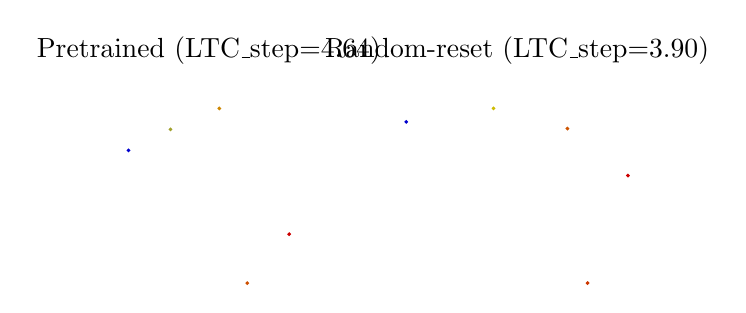
\begin{tikzpicture}
\begin{groupplot}[group style={group size=2 by 1,horizontal sep=1.0cm},width=0.46\linewidth,height=0.35\linewidth,axis equal image,axis lines=none]
\nextgroupplot[title={Pretrained (LTC\_step=4.64)}]\addplot+[only marks,mark=*,mark size=0.45pt,scatter,scatter src=x] coordinates {(-1.2,0.8) (-0.6,1.1) (0.1,1.4) (1.1,-0.4) (0.5,-1.1)};
\nextgroupplot[title={Random-reset (LTC\_step=3.90)}]\addplot+[only marks,mark=*,mark size=0.45pt,scatter,scatter src=x] coordinates {(-1.6,1.2) (-0.3,1.4) (0.8,1.1) (1.7,0.4) (1.1,-1.2)};
\end{groupplot}
\end{tikzpicture}

\end{document}
